\documentclass[xcolor=svgnames]{beamer}
\usetheme[
    %%% options passed to the outer theme
    %    hidetitle,           % hide the (short) title in the sidebar
    %    hideauthor,          % hide the (short) author in the sidebar
    %    hideinstitute,       % hide the (short) institute in the bottom of the sidebar
    %    shownavsym,          % show the navigation symbols
         width=1.5cm,         % width of the sidebar (default is 2 cm)
    %    hideothersubsections,% hide all subsections but the subsections in the current section
    %    hideallsubsections,  % hide all subsections
         left                 % right of left position of sidebar (default is right)
    %%% options passed to the color theme
        lightheaderbg         % use a light header background
  ]{AAUsidebar}

% #### graphics and schemes
\usepackage{graphicx}
\graphicspath{{img/}}
\usepackage{tikz}
\usetikzlibrary{                          % TikZ libraries
                scopes,                   % .
                shapes,                   % .
                arrows,                   % .
                through,                  % .
                calc,                     % .
                intersections,            % .
                spy,                      % .
                matrix,                   % .
                chains,                   % .
                decorations.pathreplacing,% .
                decorations.pathmorphing, % .
                decorations.markings}     % .

\usepackage{pgfplots}                     % TikZ plots
\usepackage{pgfplotstable}                % TikZ tables from CSV
\pgfplotsset{compat=1.3}                  % activates \xilabel shift` for pgfplots
\usepackage{array}
\usepackage{listings}
\usepackage{ccicons}
\usepackage{tcolorbox}
\usepackage{listings}                     % code
\usepackage{adjustbox}                    % code
\usepackage{eurosym}                      % euro symbol
\usepackage{attrib}

% #### colors
\usepackage{xcolor}                       % common color names
\usepackage{colortbl}                     % common color names

% #### layouts
\usepackage{multicol}
\usepackage[textfont=footnotesize,bf]{caption}
\usepackage{subfig}

% #### math
\usepackage{siunitx}

% #### fonts
\usepackage[utf8]{inputenc}
\usepackage[english]{babel}
\usepackage[T1]{fontenc}
\usepackage{cmbright}
\usepackage{soul} %slanted text
\usepackage{hyperref}
\urlstyle{same}
\hypersetup{pdfauthor={Francesco de Virgilio},pdftitle={Handling GRIB files: when NOT to use GIS to manage geographic data}}

% #### tables
\usepackage{booktabs}			          % migliora la qualità delle tabelle
\usepackage{tabularx}			          % colonne a spaziatura fissa delle tabelle
\newcommand{\otoprule}                    % better top rule horizontal line
    {\midrule[\heavyrulewidth]}           % .


\begin{document}

\usebackgroundtemplate{%
    
\includegraphics[width=\paperwidth,height=\paperheight]{img/back_first}}

    \begin{frame}[plain,noframenumbering]
        \begin{center}
            \color{white}
            \LARGE{Handling weather GRIB files}\\
            \normalsize{When \textit{not} to use GIS to manage geographic data}\\
            \vspace{40pt}
            Francesco de Virgilio\\
            \vspace{8pt}
            \scriptsize{Pole Star Space Applications}\\
            \scriptsize{London, 27 Jan 2015}
        \end{center}
    \end{frame}

\usebackgroundtemplate{%
    
\includegraphics[width=\paperwidth,height=\paperheight]{img/back_normal}}

\section{GIS}

    \begin{frame}{GIS in Pole Star}
        \begin{center}
            \color{black}
            \begin{block}{Geographic Information System}
                Is a computer system designed to capture, store, manipulate, analyze, manage, and present all types of spatial or geographical data.
            \end{block}
        \end{center}
        \vspace{0.05\textheight}
        \only<2->{Extensions to well-known software}
        \begin{columns}[c]
            \column{.5\textwidth}
                \begin{itemize}
                    \item<2-> Django
                    \item<3-> PostgreSQL
                \end{itemize}
            \column{.5\textwidth}
                \begin{itemize}
                    \item<2-> geoDjango
                    \item<3-> PostGIS
                \end{itemize}
        \end{columns}
    \end{frame}

   \subsection{Why GIS?}

   % * functions to ease some calculations
   % * quicker data retrieval and analysis

        \begin{frame}
        \end{frame}
 
    \subsection{Impracticalities}

    % * different packages, need to match different versions
    % * lack of support for some formats

        \begin{frame}
        \end{frame}

\section{Weather}

    \subsection{Objective}

        \begin{frame}{Target}
            \begin{block}{CAS-179: Weather API}
                Take in the GRIB file, and provide an internal API, that can give weather info for a given time/lat/lon.
            \end{block}
            \vfill
            \pause
            Example:\\
            \begin{center}
                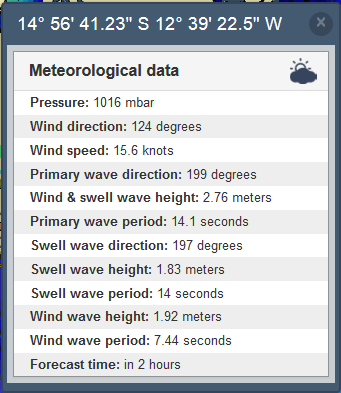
\includegraphics[width=0.35\textwidth]{img/weather_pufi}
            \end{center}
        \end{frame}

    \subsection{GRIB data}
    % * data specification

        \begin{frame}{GRIB file format in a nutshell}
            \begin{columns}[c]
                \column{.5\textwidth}
                \onslide<1->{
                    \small
                    \begin{itemize}
                        \item GRIB: \textbf{G}eneral \textbf{R}egularly-distributed \textbf{I}nformation in \textbf{B}inary form
                        \item current data provider: Tidetech Pty Ltd
                        \item updated every day
                        \item average file dimension: 39 Mb
                        \item 17 layers
                        \item timespan: 6 days
                        \item covered area: whole planet
                    \end{itemize}
                }
                \column{.5\textwidth}
                \onslide<2->{
                    \scriptsize
                    \begin{itemize}
                        \item \temporal<3>{latitudes array (-90, +90)}{\textbf{latitudes array (-90, +90)}}

                        \item \temporal<3>{longitudes array (-180, +180)}{\textbf{longitudes array (-180, +180)}}

                        \item minutes from first observation
                        \item string with datetime
                        \item initial\_time3\_hours (time)
                        \item PeakWaveDirection
                        \item SignificantWaveHeight
                        \item PressureReduced0SL
                        \item PeakWavePeriod
                        \item SwellWavesMeanPeriod
                        \item SwellWavesSignificantHeight
                        \item SwellWavesDirection
                        \item WindUComponent
                        \item WindVComponent
                        \item WindWavesMeanPeriod
                        \item WindWavesSignificantHeight
                    \end{itemize}
                }
            \end{columns}
        \end{frame}

        \begin{frame}{Show me a GRIB! \small{(1 layer)}}
            \begin{figure}
                \centering
                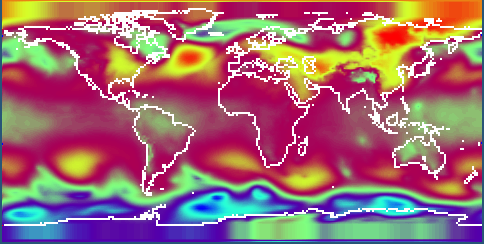
\includegraphics[width=0.8\textwidth]{img/nc_screen}
                \caption{Pressure Reduced at mean sea level, Tidetech data}
                \label{fig:prmsl}
            \end{figure}
        \end{frame}

    \subsection{PurpleFinder}
    % * old approach: PuFi

        \begin{frame}{Old approach: PurpleFinder}
        \end{frame}

    \subsection{NumPy}
    % * new approach: NumPy parsing + API

        \begin{frame}{Current approac: NumPy NetCDF parsing}
        \end{frame}

    \subsection{PostGIS 2}
    % * future approach: PostGIS raster + API

        \begin{frame}{Future approach: PostGIS 2 raster}
        \end{frame}

\section{Space: grid}

    \begin{frame}
    \end{frame}

\section{Time: slots}

    \begin{frame}
    \end{frame}

\section{Response structure}

    \begin{frame}
    \end{frame}

\section{Thanks}

    \begin{frame}
    \end{frame}

\section{Questions?}
% https://www.flickr.com/photos/nikokahkonen/3884840445

    \begin{frame}
    \end{frame}

\end{document}
